\chapter{信号与系统}

学习要点:

\begin{itemize}
    \item 认识本课程领域的一些名词、术语。
    \item 学习信号运算规律、熟悉表达式与波形的对应关系。
    \item 理解冲激信号的特性
    \item 了解本课程研究范围、学习目标
    \item 初步了解本课程用到的主要方法和手段
\end{itemize}

\section{绪论}

\subsection{信号的概念}
信号\footnote{指电信号}是\uwave{信息的载体}

辨析:
\begin{itemize}
    \item 消息:人们常常把来自外界的各种报道统称为消息。
    \item 信息\footnote{本课程中对“信息”和“消息”两词不加严格区分}:通常把消息中有意义的内容称为信息。
    \item 信号:信号是信息的载体,通过信号传递信息。
\end{itemize}

\subsection{系统的概念}

\begin{Figure}[系统组成]
    
\includegraphics[width=100mm]{visio/1.1.pdf}
\end{Figure}

信号处理:对信号进行加工/变换

信号传输:通信(长距离)



\section{信号的描述和分类}

\subsection{信号的描述}

信号:信息的物理体现,随时间变化

分类:电信号/非电信号

基本形式:随时间变化的电压$v(t)$/电流$i(t)$\footnote{本课程内不区分电压信号和电流信号}

描述:时间的函数\footnote{本课程内信号和函数说法上等价},图形表示为波形

\subsection{信号的分类}

\begin{itemize}
    \item 用途:电视信号/雷达信号\dots
    \item 时间特性:确定/随机信号、连续\footnote{时间和幅值均连续}/离散\footnote{时间和幅值均离散,又称序列}信号、模拟/数字信号、周期/非周期信号、能量/功率信号\dots
\end{itemize}

\subsubsection{连续信号和离散信号}

\begin{Figure}[连续信号]
    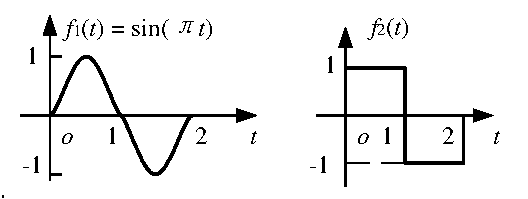
\includegraphics[width=80mm]{visio/1.2.pdf}
\end{Figure}

对于连续时间信号,其要求定义域连续,可包含间断点,值域可以不连续

\begin{Figure}[离散信号]
    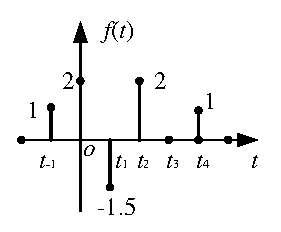
\includegraphics[width=40mm]{visio/1.3.pdf}
\end{Figure}

对于离散信号,其仅在离散时刻有定义,且离散点间隔可以不等,通常取间隔$T$,表示为$f(kT)$,简写为$f(k)$。

等间隔的离散信号称为序列,其中$k$为序号。

\xref{fig:离散信号}可以表示为以下形式:

\begin{equation}
    f(k)=\left\{
    \begin{aligned}
        1    & , & k=-1         \\
        2    & , & k=0          \\
        -1.5 & , & k=1          \\
        2    & , & k=2          \\
        0    & , & k=3          \\
        1    & , & k=4          \\
        0    & , & \text{其他}k
    \end{aligned}
    \right.
\end{equation}

\subsubsection{模拟信号、抽样信号和数字信号}

\begin{Figure}[模拟、抽样、数字信号]
    \begin{FigureSub}[模拟信号]
        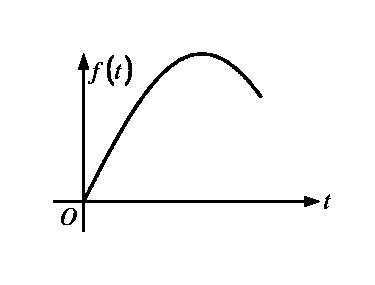
\includegraphics[width=40mm]{visio/1.4-a.pdf}
    \end{FigureSub}
    \begin{FigureSub}[抽样后信号]
        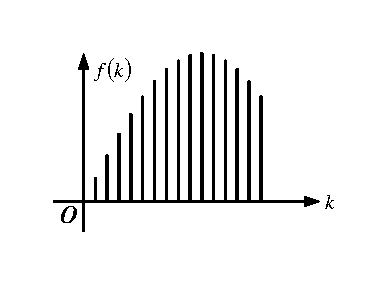
\includegraphics[width=40mm]{visio/1.4-b.pdf}
    \end{FigureSub}
    \begin{FigureSub}[数字信号]
        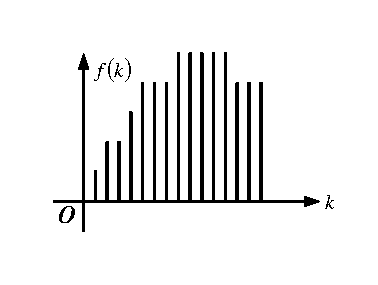
\includegraphics[width=40mm]{visio/1.4-c.pdf}
    \end{FigureSub}
\end{Figure}

对于模拟信号,其时间和幅值均连续,是连续时间信号,经过抽样后变换为抽样信号。

抽样信号时间离散但幅值连续,经过量化后变换为数字信号。

数字信号时间和幅值均离散,是离散时间信号。

\subsubsection{周期信号}

\begin{BoxDefinition}[周期信号]*
    定义在$(-\infty,\infty)$区间,每隔一定时间$T$(或整数$N$),按相同规律重复变化的信号。

    连续周期信号$f(t)$满足
    \begin{Equation}
        f(t) = f(t+mT), m=0,\pm 1,\pm 2,\dots
    \end{Equation}
    离散周期信号$f(t)$满足
    \begin{Equation}
        f(k) = f(k+mN), m=0,\pm 1,\pm 2,\dots
    \end{Equation}

    满足上述关系的最小$T$(或整数$N$)称为该信号的周期。
\end{BoxDefinition}

不具有周期性的信号称为非周期信号。

\begin{BoxProperty}[连续周期信号的周期]*
    两个周期信号$x(t),y(t)$的周期分别为$T_1$和$T_2$,若其周期之比$T_1/T_2$为有理数,则其和信号$x(t)+y(t)$仍然是周期信号,其周期为$T_1$和$T_2$的最小公倍数。
\end{BoxProperty}

\begin{BoxProperty}[正弦序列的周期]*
    对于离散周期信号$f(k) = \sin(\beta k)$。

    仅当$\frac{2\pi}{\beta}$为整数时,正弦序列才具有周期
    \begin{Equation}
        N=\frac{2\pi}{\beta}
    \end{Equation}
    当$\frac{2\pi}{\beta}$为有理数时,正弦序列仍具有周期性,其周期为
    \begin{Equation}
        N=M\cdot\frac{2\pi}{\beta}
    \end{Equation}
    其中$M$取使$N$为整数的最小整数。

    当$\frac{2\pi}{\beta}$为无理数时,为非周期序列。
\end{BoxProperty}

容易得知,两个周期信号的和不一定是周期信号,但两周期序列之和一定是周期序列。

\subsubsection{能量信号和功率信号}

\begin{BoxDefinition}[能量信号]*
    满足以下条件的连续信号称为能量信号
    \begin{Equation}
        E = \int_{-\infty}^{\infty}\left|f(t)\right|^2 dt < \infty
    \end{Equation}
    满足以下条件的离散信号称为能量信号
    \begin{Equation}
        E = \sum\limits_{k=-\infty}^{\infty}\left|f(k)\right|^2 < \infty
    \end{Equation}
    即能量有界,此时有$P = 0$
\end{BoxDefinition}

\begin{BoxDefinition}[功率信号]*
    满足以下条件的连续信号称为功率信号
    \begin{Equation}
        P = \lim_{T \rightarrow \infty} \frac{1}{T} \int_{-\frac{T}{2}}^{\frac{T}{2}}\left|f(t)\right|^2 dt < \infty
    \end{Equation}
    满足以下条件的离散信号称为功率信号
    \begin{Equation}
        P = \lim_{N \rightarrow \infty} \frac{1}{N} \sum\limits_{k=-\frac{N}{2}}^{\frac{N}{2}}\left|f(k)\right|^2 < \infty
    \end{Equation}
    即功率有界,此时有$E = \infty$
\end{BoxDefinition}

一般周期信号为功率信号,时限信号\footnote{有限时间区间不为零的非周期信号}为能量信号。

一些非周期信号也是非能量信号,例如:$\varepsilon (t)$ 是功率信号,$t\varepsilon (t)$、$e^t$是非功率非能量信号,$\delta (t)$是无定义的非功率非能量信号。

\subsubsection{一维信号和多维信号}

\begin{BoxDefinition}[一维信号]*
    只由一个自变量描述的信号,如语音信号。
\end{BoxDefinition}

\begin{BoxDefinition}[多维信号]*
    由多个自变量描述的信号,如图像信号。
\end{BoxDefinition}

\subsection{几种典型确定性信号}

\subsubsection{指数信号}

\begin{Figure}[指数信号]
    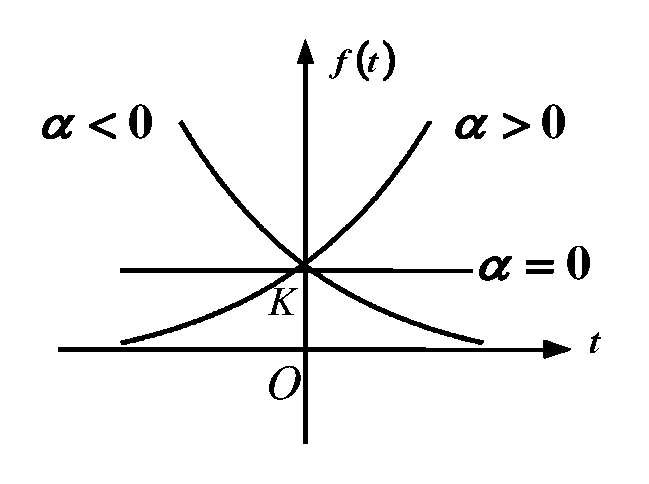
\includegraphics[width=40mm]{visio/1.5.pdf}
\end{Figure}

\begin{BoxDefinition}[指数信号]*
    形如以下形式的信号为指数信号
    \begin{Equation}
        f(t)=Ke^{\alpha t}
    \end{Equation}
    $\alpha = 0$时为直流(常数)

    $\alpha < 0$时指数衰减

    $\alpha > 0$时指数增长
\end{BoxDefinition}

\begin{BoxDefinition}[单边衰减指数信号]*
    \begin{Equation}
        f(t)=\left\{
        \begin{aligned}
            0    & , &t<0 \\
            e^{-\frac{t}{\tau}}    & , &t \geq 0
        \end{aligned}
        \right.
    \end{Equation}
    时间常数,代表信号的衰减速度
    \begin{Equation}
        \tau = \frac{1}{|\alpha|}
    \end{Equation}
\end{BoxDefinition}


\subsubsection{正弦信号}

\begin{BoxDefinition}[正弦信号]*
    形如以下形式的信号为正弦信号
    \begin{Equation}
        f(t)=K\sin(\omega t +\theta)
    \end{Equation}
    周期
    \begin{Equation}
        T = \frac{2\pi}{\omega}
    \end{Equation}
    角频率
    \begin{Equation}
        \omega = 2\pi f
    \end{Equation}
\end{BoxDefinition}

\begin{BoxDefinition}[衰减正弦信号]*
    \begin{Equation}
        f(t)=\left\{
        \begin{aligned}
            Ke^{-\alpha t}\sin(\omega t)    & , &t\geq 0 \\
            0    & , &t < 0
        \end{aligned}
        \right.
        \quad (\alpha > 0)
    \end{Equation}
\end{BoxDefinition}

\subsubsection{复指数信号}

\begin{BoxDefinition}[复指数信号]*
    复指数信号
    \begin{Equation}
        f(t)=Ke^{(\sigma + \mathrm{j} \omega)t}=Ke^{\sigma t}\cos(\omega t) + \mathrm{j}Ke^{\sigma t}\sin(\omega t)
    \end{Equation}
    复频率
    \begin{Equation}
        s=\sigma + \mathrm{j} \omega
    \end{Equation}
    其中$\sigma$的量纲为$1/s$,$\omega$的量纲为$rad/s$
\end{BoxDefinition}

特点:不能产生,用来描述各种信号,用于信号分析及运算简化。

当$\sigma = 0, \omega = 0$时,为直流信号

当$\sigma > 0, \omega = 0$时,为升指数信号

当$\sigma < 0, \omega = 0$时,为衰减指数信号

当$\sigma = 0, \omega \neq 0$时,为等幅振荡

当$\sigma > 0, \omega \neq 0$时,为增幅振荡

当$\sigma < 0, \omega \neq 0$时,为衰减振荡

\subsubsection{抽样信号}

\begin{Figure}[抽样信号]*
    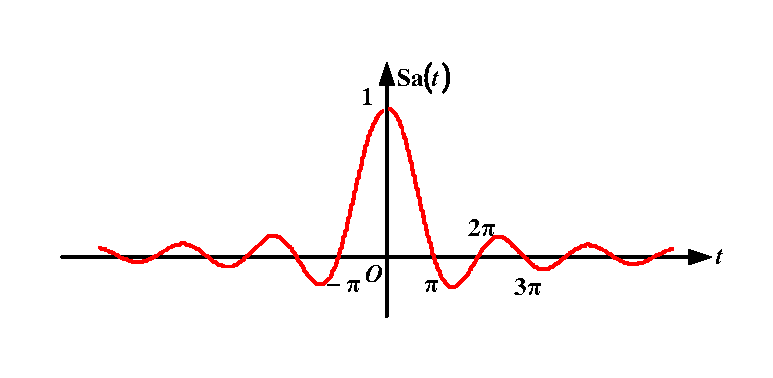
\includegraphics[width=100mm]{visio/1.6.pdf}
\end{Figure}

\begin{BoxDefinition}[抽样信号]
    抽样信号
    \begin{Equation}
        Sa(t)=\frac{\sin t }{t}
    \end{Equation}
\end{BoxDefinition}

\begin{BoxProperty}[抽样信号的性质]*
    抽样信号有如下性质
    \begin{Equation}
        \begin{array}{l}
            Sa(-t) = Sa(t) \\
            t=0,Sa(t)=1 \quad (\lim\limits_{t\rightarrow 0}Sa(t)=1)\\
            Sa(t)=0, t=\pm n\pi, n=1,2,3\cdots \\
            \int_0^{\infty}\frac{\sin t}{t}dt = \frac{\pi}{2}, \int_{-\infty}^{\infty}\frac{\sin t}{t}dt=\pi \\
            \lim\limits_{t\rightarrow\pm\infty}Sa(t)=0\\
            \mathrm{sinc}(t)=\frac{\sin(\pi t)}{\pi t}
        \end{array}
    \end{Equation}
    
\end{BoxProperty}


\section{信号的基本运算}

\subsection{信号的加法和乘法}

同一瞬时两信号对应值相加(相乘)

离散序列相加、乘对应值相加(相乘)

\subsection{信号的时间变换}

\subsubsection{信号的反转}

\begin{Figure}[信号的反转]
    \begin{FigureSub}[反转前原始信号$f(t)$]
        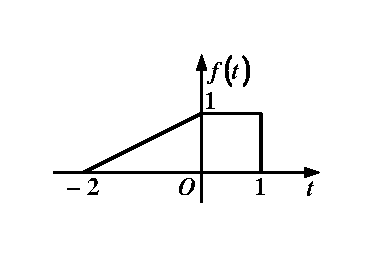
\includegraphics[width=40mm]{visio/1.7-a.pdf}
    \end{FigureSub}
    \begin{FigureSub}[反转信号$f(-t)$]
        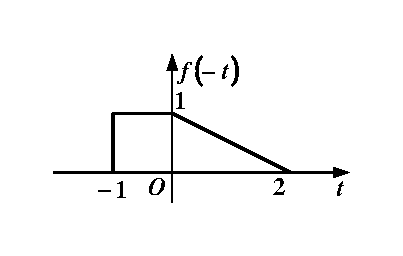
\includegraphics[width=40mm]{visio/1.7-b.pdf}
    \end{FigureSub}
\end{Figure}

\begin{BoxDefinition}[信号的反转]
    将$f(t)\rightarrow f(-t),f(k)\rightarrow f(-k)$称为对信号$f(\cdot)$的反转或反折。
\end{BoxDefinition}

\subsubsection{信号的平移}

\begin{Figure}[信号的平移]
    \begin{FigureSub}[平移前原始信号$f(t)$]
        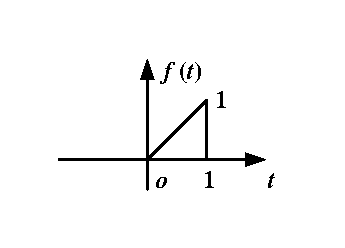
\includegraphics[width=40mm]{visio/1.8-a.pdf}
    \end{FigureSub}
    \begin{FigureSub}[平移信号$f(t-1)$]
        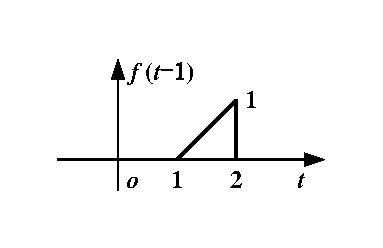
\includegraphics[width=40mm]{visio/1.8-b.pdf}
    \end{FigureSub}
\end{Figure}

\begin{BoxDefinition}[信号的平移]
    将$f(t)\rightarrow f(t-t_0),f(k)\rightarrow f(k-k_0)$称为对信号$f(\cdot)$的平移。

    若$t_0$(或$k_0$)$>0$,则将$f(\cdot)$右移,否则左移。
\end{BoxDefinition}

\subsubsection{信号的展缩}

\begin{Figure}[信号的展缩]
    \begin{FigureSub}[压缩前原始信号$f(t)$]
        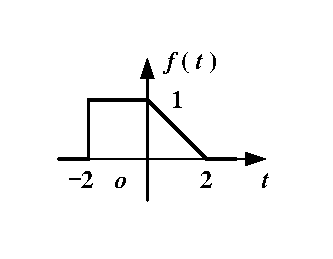
\includegraphics[width=40mm]{visio/1.9-a.pdf}
    \end{FigureSub}
    \begin{FigureSub}[压缩信号$f(2t)$]
        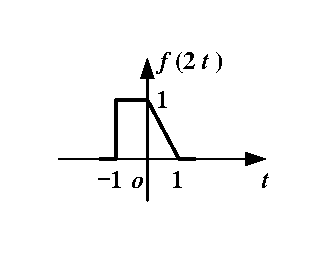
\includegraphics[width=40mm]{visio/1.9-b.pdf}
    \end{FigureSub}
\end{Figure}


\begin{BoxDefinition}[信号的展缩]
    将$f(t)\rightarrow f(at)$称为对信号$f(t)$的尺度变换。

    若$a>1$,则波形沿横坐标压缩。

    若$0<a<1$,则扩展。
\end{BoxDefinition}

离散信号一般不作尺度变换。

\subsubsection{信号的混合运算}

对正向运算$f(t)\rightarrow f(at+b)$,先平移再展缩最后再反转。

对逆向运算$f(at+b)\rightarrow f(t)$,先反转展缩,最后平移。

\subsection{信号的微分和积分}

\begin{Figure}[信号的微分]
    \begin{FigureSub}[微分前原始信号]
        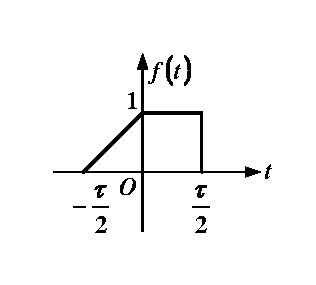
\includegraphics[width=40mm]{visio/1.10-a.pdf}
    \end{FigureSub}
    \begin{FigureSub}[信号微分]
        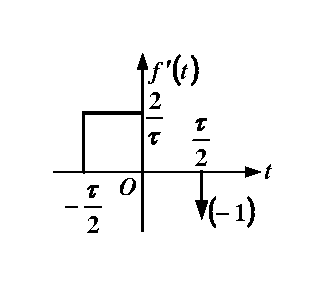
\includegraphics[width=40mm]{visio/1.10-b.pdf}
    \end{FigureSub}
\end{Figure}

\begin{Figure}[信号的积分]
    \begin{FigureSub}[积分前原始信号]
        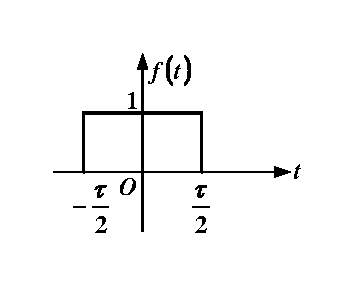
\includegraphics[width=40mm]{visio/1.11-a.pdf}
    \end{FigureSub}
    \begin{FigureSub}[信号积分]
        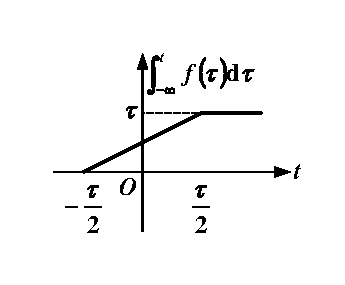
\includegraphics[width=40mm]{visio/1.11-b.pdf}
    \end{FigureSub}
\end{Figure}
\section{阶跃函数和冲激函数}
函数本身有不连续点(跳变点)或其导数与积分有不连续点的一类函数统称为奇异信号或奇异函数。
\subsection{单位阶跃函数}

\begin{Figure}[单位阶跃函数]
    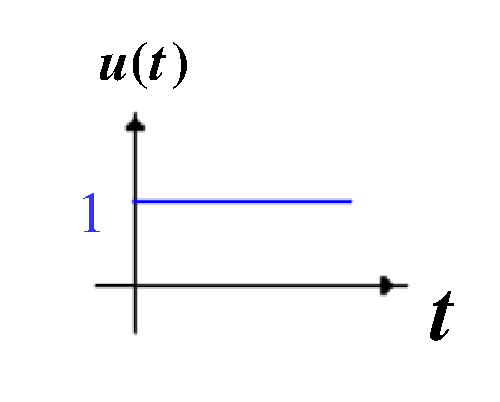
\includegraphics[width=40mm]{visio/1.12.pdf}
\end{Figure}

\begin{BoxDefinition}[单位阶跃函数]
    单位阶跃函数
    \begin{Equation}
        u(t)=\left\{
        \begin{aligned}
            1 & , & t > 0 \\
            0 & , & t < 0
        \end{aligned}
        \right.
    \end{Equation}
    $t=0$处发生跳变,或认为$u(t)=\frac{1}{2}$
\end{BoxDefinition}

对单位阶跃函数作平移可得延迟单位阶跃信号。

\begin{BoxProperty}[单位阶跃函数的性质]
    可以通过平移和加减运算表示某些函数

    可以表示某些函数的区间(乘上阶跃函数的组合)

    阶跃函数的积分

    \begin{Equation}
        \int_{-\infty}^{t} \varepsilon(\tau) d\tau = t\varepsilon(t)
    \end{Equation}
\end{BoxProperty}

\subsection{单位冲激函数}

\begin{Figure}[单位冲激函数]
    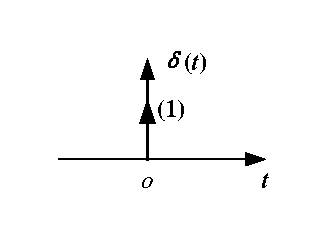
\includegraphics[width=40mm]{visio/1.13.pdf}
\end{Figure}

\begin{BoxDefinition}[单位冲激函数]
    设一矩形脉冲$p_{\tau}(t)$的宽为$\tau$,高为$\frac{1}{\tau}$,面积为$1$
    \begin{Equation}
        \delta(t) = \lim\limits_{\tau\rightarrow 0} p_{\tau}(t)
    \end{Equation}
    或由狄拉克定义
    \begin{Equation}
        \left\{
        \begin{array}{ll}
            \delta (t) = 0 & (t \neq 0) \\
            \int_{-\infty}^{\infty} \delta (t)dt=1
        \end{array}
        \right.
    \end{Equation}
    且
    \begin{Equation}
        \int_{-\infty}^{\infty} \delta (t)dt= \int_{0_{-}}^{0_{+}} \delta (t)dt = 1
    \end{Equation}
    $t=0$时,$\delta(t)\rightarrow \infty$,为无界函数。
\end{BoxDefinition}

\subsection{冲激函数的性质}

\begin{BoxProperty}[冲激函数的取样性]
    冲激函数的取样性
    \begin{Equation}
        f(t)\delta(t)=f(0)\delta(t) \\
    \end{Equation}
    \begin{Equation}
        \int_{-\infty}^{\infty} f(t)\delta(t)dt = f(0)
    \end{Equation}
\end{BoxProperty}

\begin{BoxProperty}[冲激函数的奇偶性]
    冲激函数为偶函数
    \begin{Equation}
        \delta(-t)=\delta(t)
    \end{Equation}
\end{BoxProperty}

\begin{BoxProperty}[冲激函数的比例性]
    冲激函数的展缩变换有以下性质
    \begin{Equation}
        \delta(at)=\frac{1}{|a|}\delta(t)
    \end{Equation}
    结合平移
    \begin{Equation}
        \delta(at-t_0)=\frac{1}{|a|}\delta(t-\frac{t_0}{a})
    \end{Equation}
\end{BoxProperty}

\begin{BoxProperty}[冲激函数的微积分性质]
    冲激函数与阶跃函数有以下关系
    \begin{Equation}
        \varepsilon (t) = \int_{-\infty}^{t} \delta (\tau) d\tau
    \end{Equation}
    或
    \begin{Equation}
        \delta (t) = \frac{d\varepsilon(t)}{dt}
    \end{Equation}
\end{BoxProperty}

引入冲激函数后,间断点导数也连续。

\begin{BoxProperty}[复合函数形式的冲激函数]
    设$f(t)$有$n$个不相等的实根$t_i(i=1,2,\dots,n)$,则
    \begin{Equation}
        \delta[f(t)]=\sum\limits_{i=1}^n\frac{1}{|f'(t_i)|}\delta(t-t_i)
    \end{Equation}
    若$f(t)$有重根,则$\delta[f(t)]$无意义。
\end{BoxProperty}

\begin{Figure}[冲激偶]
    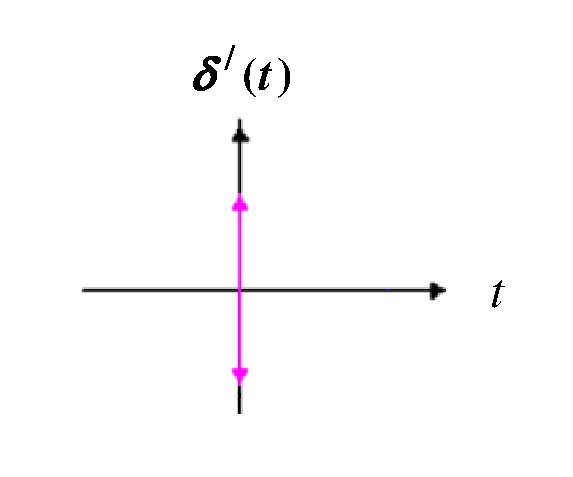
\includegraphics[width=60mm]{visio/add1.pdf}
\end{Figure}

\begin{BoxProperty}[冲激偶的性质]
    冲激偶即冲激函数的导数,有以下性质
    \begin{Equation}
        f(t)\delta'(t)=f(0)\delta'(t)-f'(0)\delta(t)
    \end{Equation}
    \begin{Equation}
        \int_{-\infty}^{\infty} f(t)\delta'(t)dt = -f'(0)
    \end{Equation}
    \begin{Equation}
        \int_{-\infty}^{t} \delta'(t)dt = \delta(t)
    \end{Equation}
    \begin{Equation}
        \int_{-\infty}^{\infty} \delta'(t)dt = 0
    \end{Equation}
    \begin{Equation}
        \delta^{(n)}(at)=\frac{1}{|a|}\cdot\frac{1}{a^n}\delta^{(n)}(t)
    \end{Equation}
\end{BoxProperty}

\subsection{单位样值序列和单位阶跃序列}

\subsubsection{单位样值序列}

\begin{Figure}[单位样值序列]
    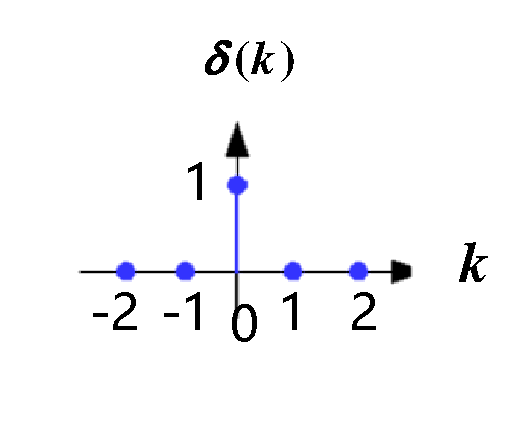
\includegraphics[width=40mm]{visio/1.14.pdf}
\end{Figure}

\begin{BoxDefinition}[单位样值序列]
    单位样值序列
    \begin{Equation}
        \varepsilon (k) \overset{\mathrm{def}}{=}
        \left\{
        \begin{aligned}
            1 & , & k = 0    \\
            0 & , & k \neq 0
        \end{aligned}
        \right.
    \end{Equation}
\end{BoxDefinition}


\begin{BoxProperty}[单位样值序列的取样性]
    单位样值序列的取样性
    \begin{Equation}
        f(k)\delta(k-k_0)=f(k_0)\delta(k-k_0)
    \end{Equation}
    \begin{Equation}
        \sum_{k=-\infty}^{\infty}f(k)\delta(k-k_0) = f(k_0)
    \end{Equation}
\end{BoxProperty}

\subsubsection{单位阶跃序列}

\begin{Figure}[单位阶跃序列]
    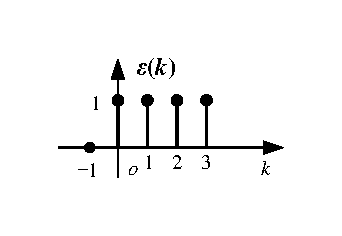
\includegraphics[width=60mm]{visio/1.15.pdf}
\end{Figure}

\begin{BoxDefinition}[单位阶跃序列]
    单位阶跃序列
    \begin{Equation}
        \varepsilon (k) \overset{\mathrm{def}}{=}
        \left\{
        \begin{aligned}
            1 & , & k \geq 0    \\
            0 & , & k < 0
        \end{aligned}
        \right.
    \end{Equation}
\end{BoxDefinition}

\begin{BoxProperty}[单位样值序列和单位阶跃序列的关系]
    单位样值序列和单位阶跃序列的关系
    \begin{Equation}
        \delta (k) = \varepsilon(k) - \varepsilon(k-1)
    \end{Equation}
    \begin{Equation}
        \varepsilon(k) = \delta(k) + \delta(k-1) + \dots
    \end{Equation}
\end{BoxProperty}



\section{系统的描述}

系统是由若干个有相互关联的单元组合而成的具有特定功能的整体。

\subsection{系统的分类}

\begin{itemize}
    \item 连续(时间)系统/离散(时间)系统/混合系统(连续和离散系统的组合)
    \item 动态系统/即时系统(记忆/无记忆系统)
\end{itemize}

\subsection{系统的数学模型}

连续系统解析描述:微分方程

离散系统解析描述:差分方程

\subsection{系统的框图描述}

\begin{Figure}[连续系统的基本单元]
    \begin{FigureSub}[加法器]
        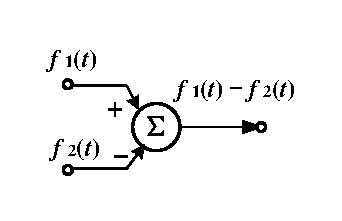
\includegraphics[width=40mm]{visio/1.16-a.pdf}
    \end{FigureSub}
    \begin{FigureSub}[乘法器]
        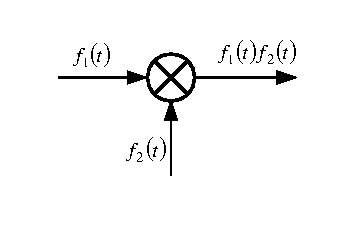
\includegraphics[width=40mm]{visio/1.16-b.pdf}
    \end{FigureSub}
    \begin{FigureSub}[积分器]
        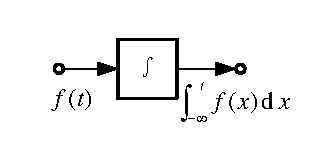
\includegraphics[width=40mm]{visio/1.16-c.pdf}
    \end{FigureSub}
    \begin{FigureSub}[延时器]
        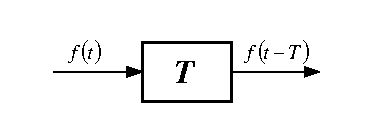
\includegraphics[width=40mm]{visio/1.16-d.pdf}
    \end{FigureSub}
    \begin{FigureSub}[数乘器]
        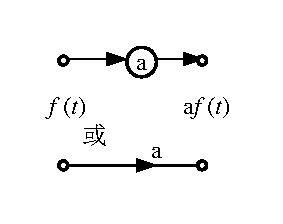
\includegraphics[width=40mm]{visio/1.16-e.pdf}
    \end{FigureSub}
\end{Figure}

微分器用积分器表示

\begin{Figure}[离散系统的基本单元]
    \begin{FigureSub}[离散系统的加法器]
        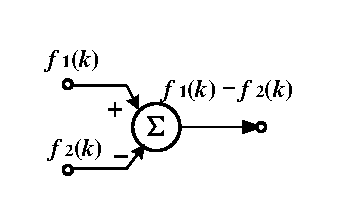
\includegraphics[width=40mm]{visio/1.17-a.pdf}
    \end{FigureSub}
    \begin{FigureSub}[离散系统的延时器]
        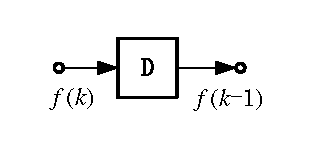
\includegraphics[width=40mm]{visio/1.17-b.pdf}
    \end{FigureSub}
    \begin{FigureSub}[离散系统的数乘器]
        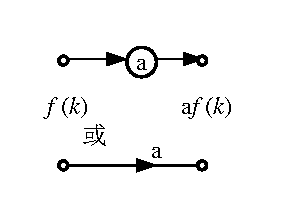
\includegraphics[width=40mm]{visio/1.17-c.pdf}
    \end{FigureSub}
\end{Figure}

根据微分方程画系统框图:

例:$ay''(t)+by'(t)+cy(t) = df'(t)+ef(t)$

设辅助函数$f(t)=ax''(t)+bx'(t)+cx(t)$

\begin{figure}[H]
    \centering
    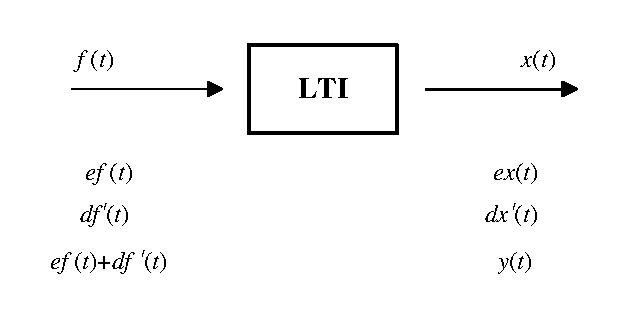
\includegraphics[width=80mm]{visio/sol1.pdf}
\end{figure}

由LTI特性:$y(t)=ex(t)+dx'(t)$

辅助函数移项可得:$x''(t)=f(t)-\frac{b}{a}x'(t)-\frac{c}{a}x(t)$


\begin{figure}[H]
    \centering
    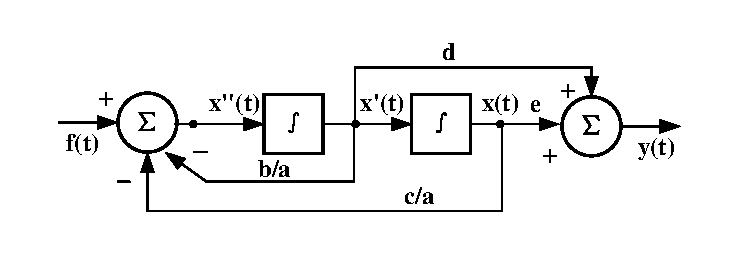
\includegraphics[width=100mm]{visio/sol2.pdf}
\end{figure}

对于框图求微分方程,逆向过程即可




\section{系统的特性与分析方法}

\subsection{系统的特性}

\subsubsection{线性}

\begin{BoxProperty}[线性系统的性质]
    设$y(\cdot)$为系统的响应,$f(\cdot)$为系统的激励,即$y(\cdot) = T[f(\cdot)]$

    齐次性
    \begin{Equation}
        f(\cdot) \rightarrow y(\cdot) \Rightarrow af(\cdot)\rightarrow ay(\cdot)
    \end{Equation}
    可加性
    \begin{Equation}
        \left\{
            \begin{aligned}
                f_1(\cdot) \rightarrow y_1(\cdot) \\
                f_2(\cdot) \rightarrow y_2(\cdot) 
            \end{aligned}
        \right.
        \Rightarrow
        f_1(\cdot) + f_2(\cdot) \rightarrow y_1(\cdot) + y_2(\cdot)
    \end{Equation}
    即线性性质
    \begin{Equation}
        af_1(\cdot) + bf_2(\cdot) \rightarrow ay_1(\cdot) + by_2(\cdot)
    \end{Equation}
\end{BoxProperty}

\begin{BoxProperty}[线性系统的条件]*
    判断一个系统是否属于线性系统,需要满足以下三个条件

    可分解性
    \begin{Equation}
        y(\cdot) = y_{zi}(\cdot)+y_{zs}(\cdot)
    \end{Equation}
    零状态线性
    \begin{Equation}
        T[\{af_1(t)+bf_2(t)\},\{0\}] = aT[\{f_1(\cdot)\},\{0\}]+bT[\{f_2(\cdot)\},\{0\}]
    \end{Equation}
    零输入线性
    \begin{Equation}
        T[\{0\},\{ax_1(0)+bx_2(0)\}] = aT[\{0\},\{x_1(0)\}]+bT[\{0\},\{x_2(0)\}]
    \end{Equation}
\end{BoxProperty}

\subsubsection{时不变性}

\begin{BoxProperty}[线性时不变系统的性质]
    线性时不变系统满足以下性质
    \begin{Equation}
        y_{zs}(t-t_d) = T[\{f(t-t_d)\},\{0\}]
    \end{Equation}
\end{BoxProperty}

直观判断方法:$f(\cdot)$前出现变系数,或有反转、展缩变换,则系统为时变系统

\subsubsection{微分与积分特性}

\begin{BoxProperty}[LTI系统的微分和积分特性]
    微分特性
    \begin{Equation}
         f(t) \rightarrow y_{zs}(t) \Rightarrow f'(t) \rightarrow y_{zs}'(t)
    \end{Equation}
    积分特性
    \begin{Equation}
         f(t) \rightarrow y_{zs}(t) \Rightarrow \int_{-\infty}^{t} f(x)dx \rightarrow \int_{-\infty}^{t} y_{zs}(t) dx
    \end{Equation}
\end{BoxProperty}

\subsubsection{因果性}
\begin{BoxDefinition}[因果系统]
    零状态响应不会出现在激励之前的系统即因果系统,即$t=t_0$时$f(t)$加入,当$t<t_0$时,$y_{zs}(t) = 0$
\end{BoxDefinition}
判断方法:输出不超前输入
\begin{BoxDefinition}[因果信号]
    $t = 0$接入系统的信号称为因果信号,可表示为$f(t)=f(t)\varepsilon(t)$
\end{BoxDefinition}

\subsubsection{稳定性}

\begin{BoxDefinition}[稳定系统]
    一个系统,若对有界的激励$f(\cdot)$所产生的零状态响应$y_{zs}(\cdot)$也是有界时,则称该系统为有界输入有界输出稳定,简称稳定。即 若$│f(\cdot)│<\infty$,其$│y_{zs} (\cdot)│<\infty$则称系统是稳定的。 
\end{BoxDefinition}

\subsection{系统的分析方法}

求解的基本思路:

\begin{itemize}
    \item 把零输入响应和零状态响应分开求。
    \item 把复杂信号分解为众多基本信号之和,根据线性系统的可加性:多个基本信号作用于线性系统所引起的响应等于各个基本信号所引起的响应之和。
\end{itemize}

采用的数学工具:
\begin{itemize}
    \item 时域:卷积积分与卷积和。
    \item 频域:傅里叶变换。
    \item 复频域:拉普拉斯变换与Z变换。
\end{itemize}